\section{Résultats numériques}

  \begin{figure}[!hbt]
    \centering
    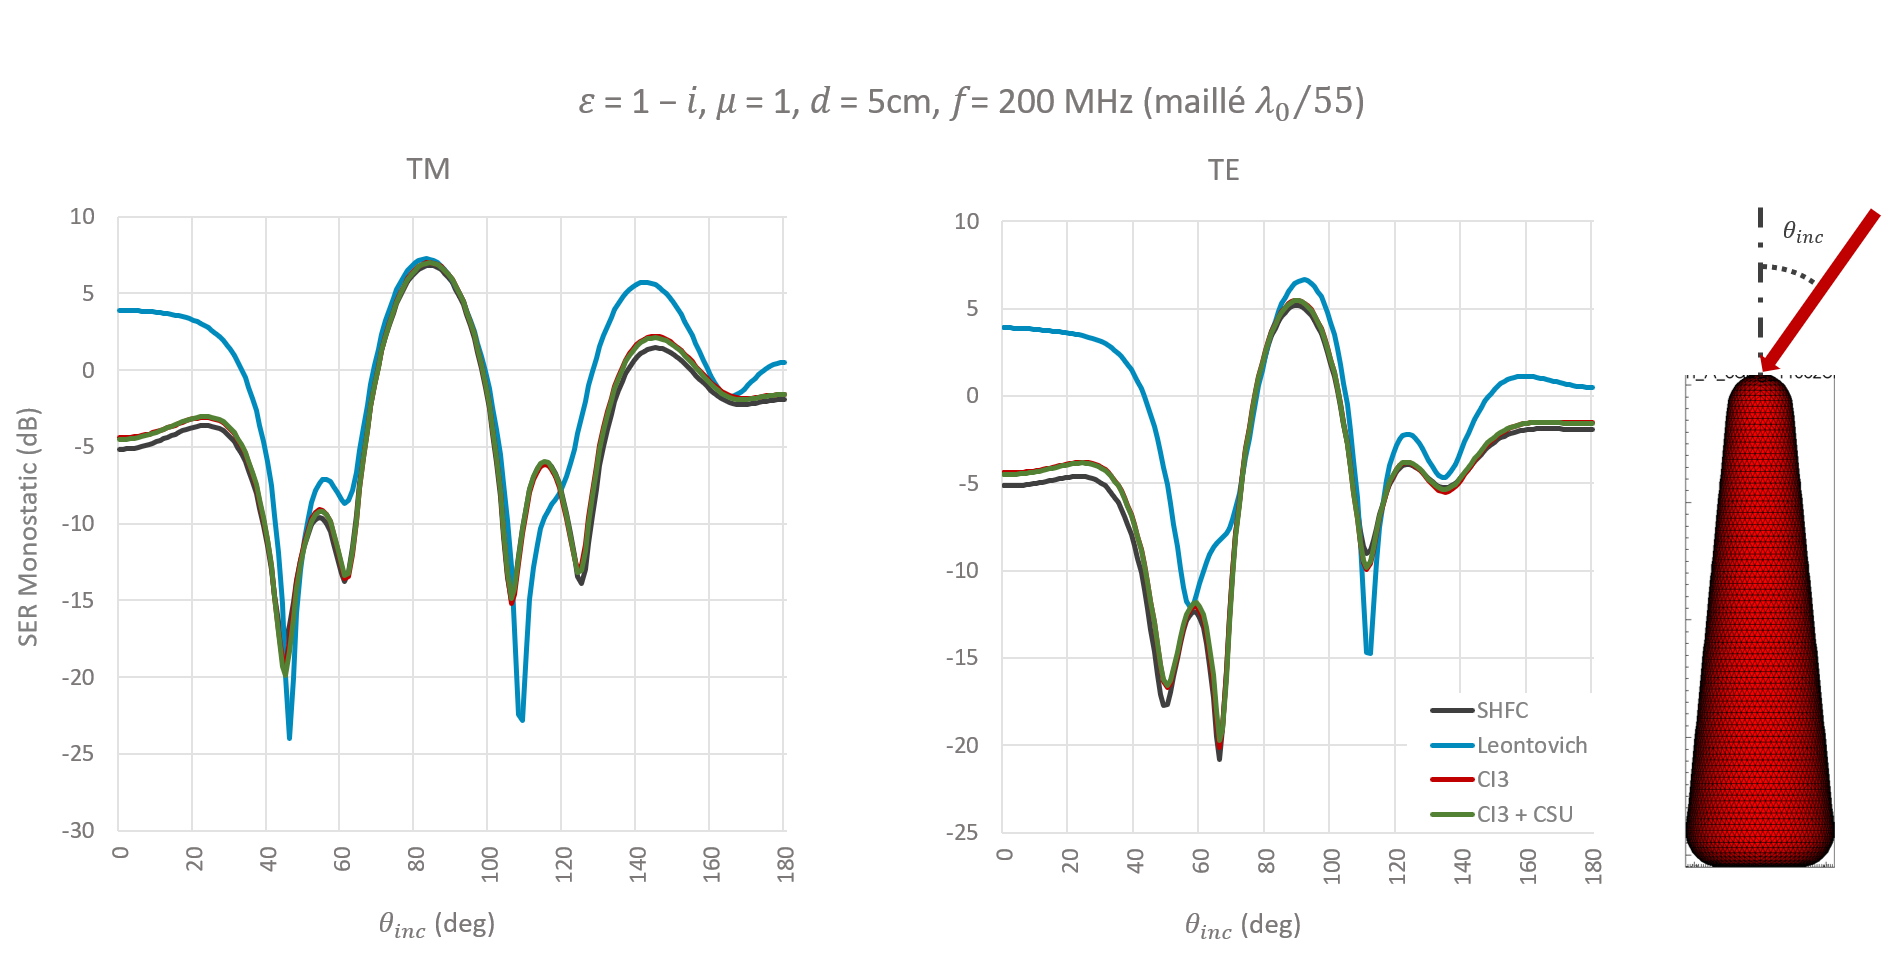
\includegraphics[width=\textwidth]{images/ser/cone_sphere_mono.png}
    \caption{SER monostatique d'un cône sphère par équations intégrales couplées avec une CIOE où les coefficients sont calculés dans le cadre de l'approximation du plan tangent.}
    \label{fig:ser:cone-sphere-mono-M1}
  \end{figure}


  \begin{figure}[!hbt]
    \centering
    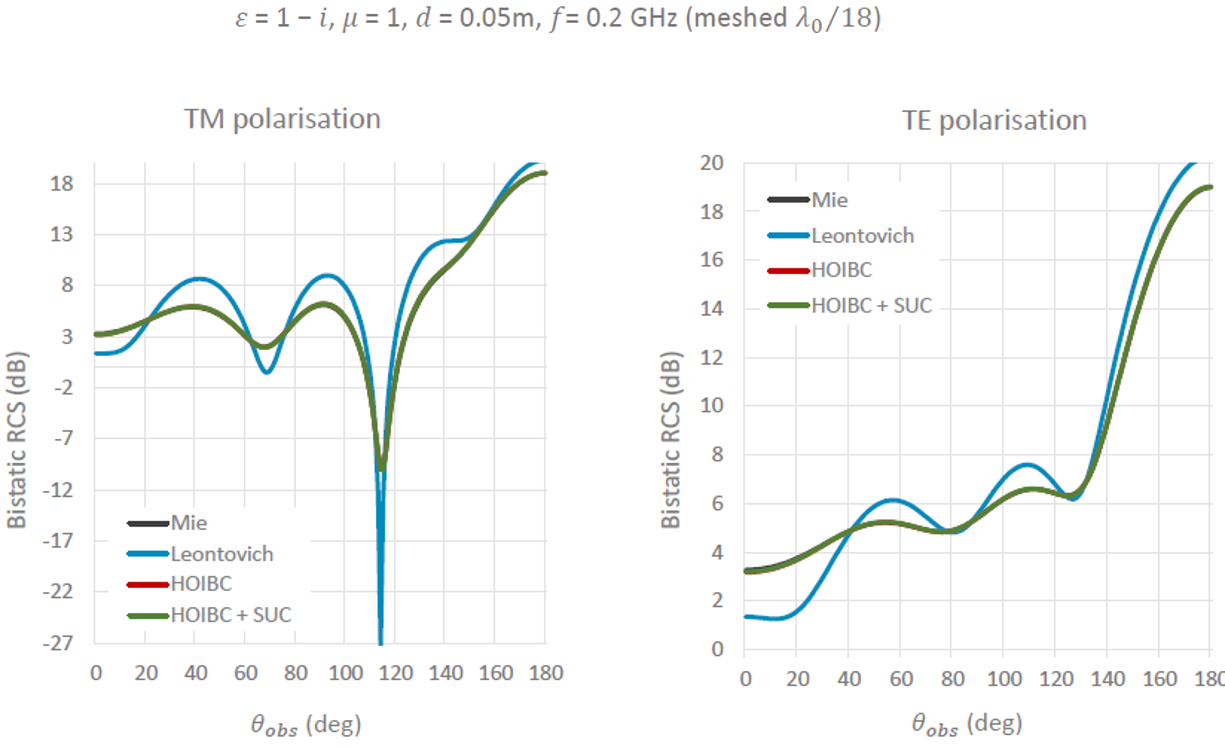
\includegraphics[width=\textwidth]{images/ser/sphere_bis.png}
    \caption{SER bistatique d'une sphère par équations intégrales couplées avec une CIOE où les coefficients sont calculés dans le cadre de l'approximation du plan tangent.}
    \label{fig:ser:sphere-bis-M1}
  \end{figure}

  Ces figures montrent que la SER calculée par EI avec CIOE est très proche de la solution de référence, calculée par un code axis symétrique de type équations intégrales avec éléments finis avec maillage des matériaux.
